\pagebreak
\subsection{Ground Support Equipment}
One personal computer will be used to connect to the E-Link through the Ethernet port. A GUI will be created to display the sensors data and a feature to change the parameters in the experiment. The GUI for the ground station shall be with MATLAB programming language and IDE.\par
The data shall be recorded and stored on the computer. 
\begin{figure}[H]
    \centering
    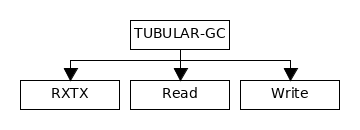
\includegraphics[width=0.6\textwidth]{4-experiment-design/img/gc-software-V1.png}
    \caption{The ground control software design tree}
    \label{fig:gcModel}
\end{figure}
The RXTX object is responsible for receiving and transmitting data over the provided Ethernet connection. The READ object takes the input received from the user, and the DISPLAY object takes data received from the RXTX object and show the data to the user through the GUI.


\raggedbottom